
\section{Structured data: the Relational Model}\label{sec:relationalcmp}
A data model is said to be \textbf{structured}\index{data!structured|textbf} if it relies on a fixed data model over which some data representation constraints are defined\footnote{Please note: some other authors like \cite{ZhangRCSWW17,Sarawagi} use the term \textit{structured} both for semistructured graph data (see Section \vref{sec:semistructured}) and relational data, both because in some cases semistructured data could be expressed in a structured fashion, and because such models are ``structured'' in comparison with unstructured data representations (see Section \vref{sec:unstructured}).}. In particular, a structured data model could be read by a domain-specific program (\textit{query}\index{query}), which can transform it or create new data expressed in the same model. The most wide spread one is the \textbf{relational model}\index{model!relational}, where data are modelled on $n$-ary mathematical relations\index{relation} $r$ \cite{RelGraph} to which a \textit{schema}\index{schema!relational model} $R$ is associated (denoted as $r(R)$). Such schema constrains the arity of the \textit{tuples}\index{tuple} $t\in r$  and the range of values that such tuples could assume. In particular, each schema $R$ is defined as $R(A_1,\dots,A_n)$, where each $A_i$ is a distinct \textit{attribute}\index{attribute|textbf} and $R$ is the name given to the relations $r$. Each relation $r(R)$ is then a subset of the cartesian product $\dom(R)\eqdef\dom(A_1)\times\dots\times \dom(A_n)$, where $\dom$ is the \textit{domain}\index{domain} function associating a set of possible values to each attribute. Consequently, each tuple may be represented within a single relation only once. In particular, each tuple $t\in r(R)$ is composed by $n$ values\footnote{This constraint will be later on called ``\textit{horizontal homogeneity''}.} $(v_1,\dots,v_n)$ such that $v_i\in \dom(A_i)$ for each\footnote{This constraint will be later on called ``\textit{vertical homogeneity}''.} $1\leq i\leq n$. A constraint, called \textbf{first normal form (1NF)}\index{first normal form|see{1NF}}\index{1NF}, provides some restrictions on the possible domains associated to such attributes: the domain  can only map attributes to sets of simple values, thus excluding tuples' values to be either sets of values \cite{Codd71a}, other relations \cite{Elmasri} or bag values.

\begin{example}
Figure \ref{fig:instance} provides an example of such data model. In particular, each table represents a relation. These are the schema of all the relations in the picture:
\[Employee(\underline{\texttt{id}},\texttt{name},\texttt{surname},\texttt{gender})\]
\[SalesOrder(\underline{\texttt{id}},\texttt{date},\texttt{deliveryDate},\texttt{orderer})\]
\[Product(\underline{\texttt{id}},\texttt{name},\texttt{category},\texttt{price})\]
\[ComposedBy(\texttt{order},\texttt{product},\texttt{quantity})\]
In particular, each row of each table represents a tuple within the relational model. 
\end{example}

\subsection{Query Languages}
Contrarily to what happens for current (graph) query languages, the first language to be developed for this data model was an algebra (called Codd's algebra or Relational Algebra \cite{atzeni,atzeniIT,Elmasri}): it investigated the most elementary operations over relations for transforming and combining them, and allowed to perform equational reasoning. As a result, equivalence rules were found, thus allowing do extract rewriting rules for obtaining equivalent queries that are more efficient than the original one provided in input. These theoretical results were used to optimize the execution of high-level denotational languages, such as SQL, by compiling them into a relational algebra representation and then performing the aforementioned optimization task.

Within this thesis we will take the knowledge of these two query languages for granted, since they are the basis for modern Relational DataBase Management Systems. %\todo{Add a reference in the appendix, explaining such query languages?}

\subsubsection{Data Mining Algebra}\label{subsec:dmalgebra}
We shall bear in mind that algebraic operators have the final aim of providing a useful tool to carry out data operations on a specific data structure (in this case, the relational model).   We shall now discuss which ``higher order'' operations are relevant in order to meet this goal. As a main reference, we now take the relational data mining algebra proposed in \cite{Calders2006}, which main concepts are sketched in Figure \ref{fig:taonta}. This algebra suggests that data in $\data$ (mainly $D_R=\emptyset$) can represent three distinct concepts: \begin{mylist}
	\item the data itself, representing some information content ($\data$),
	\item the constraints over the data ($I$), and
	\item the association to each data representation to the constraints that such data satisfies ($E$).
\end{mylist}

In particular, for each data collection $c$ represented in $\data$ ($c\in\mathcal{P}(\data)$), we want to be able to remember which elements satisfy a given property or pattern\footnote{The term used in \cite{Calders2006} is ``template''.} $p$, and provide an intermediate representation in the intensional set $I$, which elements represents an instantiation of $p$ via the elements of $c$. This operation is performed by the $\kappa_p(c)$\index{$\kappa_p$} operator.

As a next step, we would like to define a mining loop operator $\lambda$\index{$\lambda$}\index{$\lambda$|see{\texttt{fold}}} over the patterns in $I$ extracted from the data, where an expression refines such extracted patterns until such fixpoint is reached. In particular, the $\lambda$ operators are representative of a vast range of data mining algorithms, such as frequent (subgraph) mining \cite{JunghannsKAPR17} and (graph) clustering \cite{vanDongen2012} algorithms. 

Then, we want to filter out the data that satisfy such regions by associating such data elements in $D$ to the regions in $E$ ($Pop$\index{$Pop$}), and then separate the data ($\pi_A$)\index{$\pi_A$} from the satisfied properties ($\pi_{RDA}$)\index{$\pi_{RDA}$}. These two operations are required because the relational data model of interest does not allow to provide uniform data representations for both data and relations, and hence three different ``worlds'' are required. %Since graph data already provide a data representation where both data and relations coexists and that both could represent our data world, this thesis will try to extend such algebra for data mining to graph, and hence nested graphs. 

\subsection{Representation Problems}\label{sec:relreprprob}
Although most of the strengths of the relational data model rely upon a well-established theory \cite{Codd} that could be easily found on textbooks \cite{Garcia-Molina}, this model is no more up with the times. The relational model assumes a centralized structure where all the data is consolidated and under the \textsc{Closed World Assumption}\index{CWA}. On the other hand, modern data analysis techniques may also work on historical data that changes through time. Moreover, \textit{big data} forces companies to distribute the data among multiple nodes: therefore it is proved \cite{Gilbert02} that we cannot achieve strong consistency required by the relational model if we want to achieve high availability and network error tolerance. As a consequence, the model appears to be static \cite{Badia} in comparison to other approaches that allow to use open world data evolving through time. Those other approaches allow to use cooperative support \cite{Aligon201520} and to better handle schema mappings over time.  We are now going to discuss in depth some of the limitations of the relational model.


\paragraph*{Semantic Overloading}\label{subsec:semanticoverloadrel}
Each instance of a relational database can be modeled through the \textbf{Entity Relationship (ER)} model  \cite{Chen1976} using graphs; in brief, each real world entity\index{entity} is defined as a vertex (represented as squared boxes), while the relationships\index{relationship} between such entities are modelled as edges (which are represented as rhombus between the vertices). Both entities and relationships can be associated to an attribute (rendered with an oval shape). Figure \ref{fig:erschema} provides a toy example of an usage of such modelling language, where some employees can process sale orders within a company. 

As a next step, we have to transform this representation into relational tables: as we could see from Figure \ref{fig:instance}, such model is table based, and hence it does not distinguish  entities from relationships. Consequently, this whole design approach suffers from \textbf{semantic overloading}\index{semantic overloading}. Moreover, some relationships has to be expressed through \textbf{referential integrity constraints}\index{constraint!referential integrity}, and occasionally represent relationships through additional tables. In particular, {referential integrity constraints} require that every value of a \textit{foreign key} must exist as a value of a \textit{primary key} within the referred table. 

On the other hand, graphs solve the problem of the semantic overloading by representing the entities as vertices and relationships as edges as in Figure \ref{fig:graphofdb1}. On the other hand, such data model still has to implement some integrity constraints for consistency checking (e.g. when a vertex is removed, all the incoming and outgoing edges to and from that vertex has to be removed).

\paragraph*{Data Homogeneity}\label{par:homog}
Within the relational model, each tuple could be only represented within a relation and cannot have independent identification or existence. This  implies that all the relations' tuples must share the same attributes (\textbf{horizontal homogeneity})\index{homogeneity!horizontal} which must always contain values from the same domain (\textbf{vertical homogeneity})\index{homogeneity!vertical}. As a consequence, relational databases do not cope well with data under the open world assumption having a flexible and schemaless representation. 

On the other hand, the property graph model provides an ideal representation, because it does not force to represent vertices and edges into a homogeneous schema \cite{Vasilyeva13}. As showed in Figure \ref{fig:graphofdb1}, each vertex and edge shows the entity from which it cames from through its label. Moreover, no specific constraint as the relations's schema is specified for both vertices and edges, thus achieving horizontal and vertical eterogeneity.

\paragraph*{Object Identity}\label{sec:objid}
The original relational model does not formalize explicit constraints such as \textit{primary keys} identifying each tuple within a relation through a (set of) attribute(s). Those constraints can be expressed within \textsc{Relational DataBase Management Systems} (RDBMSs), thus extending the theoretical relational model. In this scenario, even if the user-defined primary key could be associated to a specific column within a table, the same key value could be still used to identify two different relational table's tuples \textit{when no specific constraint are specified}. As an example, Figure \ref{fig:instance} shows that \texttt{SalesOrder}'s id and \texttt{Product}'s id share the same primary key values, even if they refer to different instances of entities. This phenomenon does not generally arise in other graph data models (e.g. RDF\index{RDF} \cite{Allemang2011}, EPGM\index{graph!EPGM|textbf} \cite{apacheflink}%\todo{Devo aggiungere un riferimento ad un altro capitolo, dove confronto solamente i modelli a grafo tra di loro.} 
and Networks \cite{Johnson2011}), since each node is associated to an unique identifier \cite{GutierrezInclusion}, while this problem still
happens in graph databases that are based on the \textit{property graph} model, where (e.g., in Neo4J \cite{Neo4jAlg}) vertex and edge ids are used to index the graph elements, and not to univoquely identify them. 
%Consequently, the vertex indexing function is not used as an unique object identifier and it is used to provide quick access to the data resources.  

The Object Identity problem has already been formulated and solved within the Object-Oriented data model: for each object
representing an instance of a relation $\Re$, the unique identifier could be uniquely determined via a function $f_\Re$ 
(called \textit{Skolem Functor}\index{Skolem functor|textbf}\label{skolem}) which computes the unique id from the object's terms \cite{Cabibbo}. This function
generates new IDs for each newly created objects. Consequently, such objects could be easily implemented
in current programming languages (e.g. Java) where both hashing functions and equivalence predicates are provided for
each class. On the other hand, this approach does not allow to establish explicit primary keys and makes hard to retrieve the stored information. Still, the vertex and edge identifier solution could be seen as a relaxation of this Object Identification, and hence it could be adopted by the property graph such that one single set of attributes and values (and even labels) corresponds to that id.

% Besides the user-defined primary key that could be associated to a specific row, there is no independent identification of each row when conceived as an entity. As a result, modern RDBMSs allow data replication and hence conflicts could arise while updating multiple instances of the same given entity. This problem persists in the property graph model since no specific constraint are given to characterize a node as a specific entity, and consequently multiple instances of the same node could coexist. The same phenomenon happens for data represented in XML format, while RDF graphs are designed to represent each node and each labelled edge between two nodes only once. 

\paragraph*{Recursive queries}
An early extension of the relational algebra \cite{AhoAlpha} tried to introduce an algebraic operator providing a transitive closure over the directed binary relations stored in relational tables via fixpoint evaluation. As we could see from the previous discussions, the implementation of object identifiers is the main prerequisite for checking whether the tuples have been already visited or not. This fix-point operator would be later named $\alpha$ \cite{Alpha}. Recursive queries became standard with  \textbf{SQL:1999}, where a \texttt{WITH RECURSIVE} was added to the SQL syntax, and a least fix-point semantic was associated to this clause, by assuming each distinct tuple as a different object.

\begin{figure}[!pth]
	%\begin{adjustbox}{max width=\textwidth}
	\begin{minipage}[b]{\textwidth}
		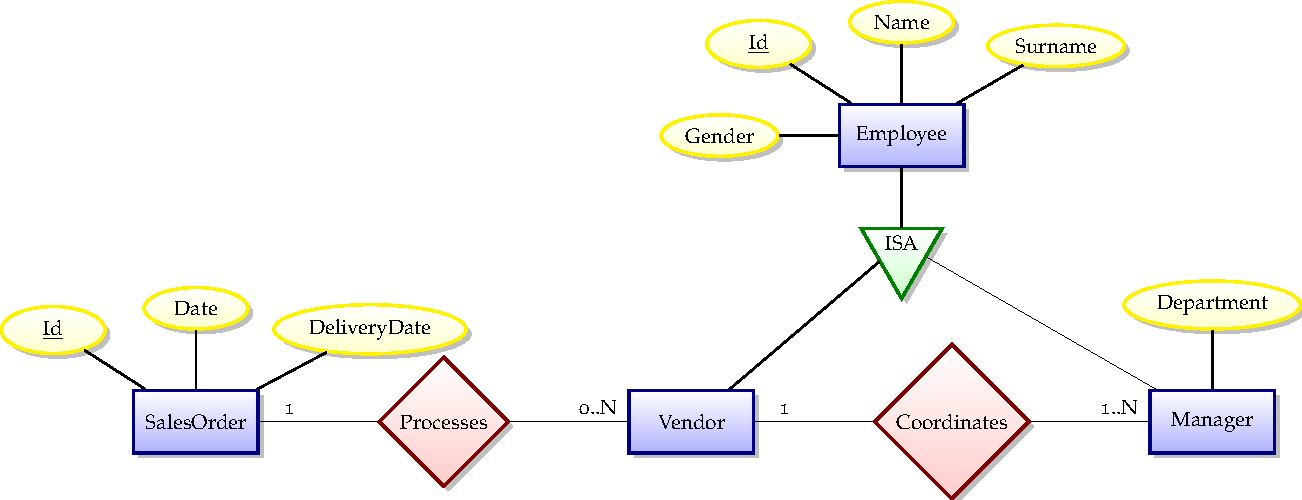
\includegraphics[scale=.6]{fig/02models/04generalization}
		\subcaption{Representing generalizations within the ER model: both vendors and managers are employees, sharing some basic attributes, except the \textit{department} information. }
		\label{fig:erISA}
	\end{minipage}\quad
	
	\begin{minipage}[b]{\textwidth}
		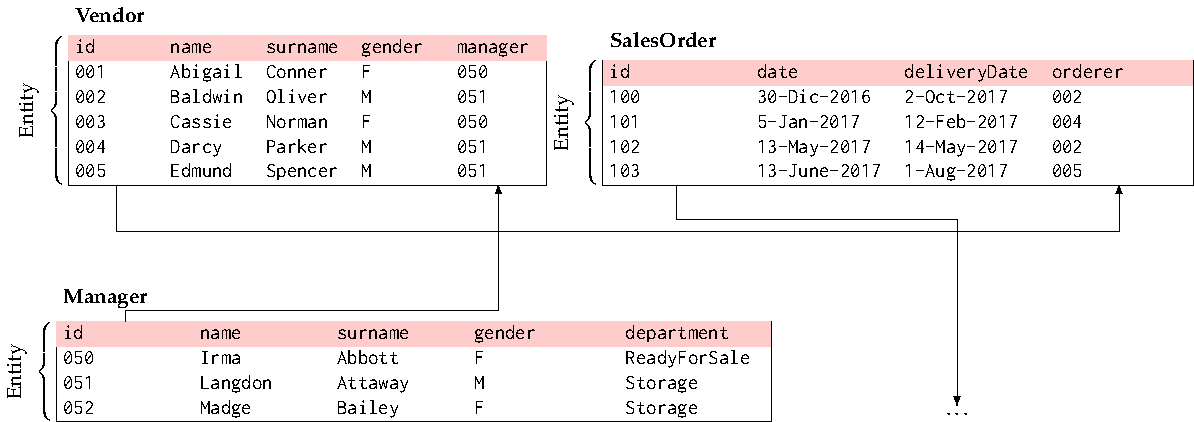
\includegraphics[scale=.7]{fig/02models/05instancegener}
		\subcaption{Vendors and Managers are represented as distinct entities. Any original information concerning the fact that both entities are \textit{Employees} is lost within the translation.}
		\label{fig:instanceRemovesIsa}
	\end{minipage}
	
	\begin{minipage}[b]{\textwidth}
		\centering
		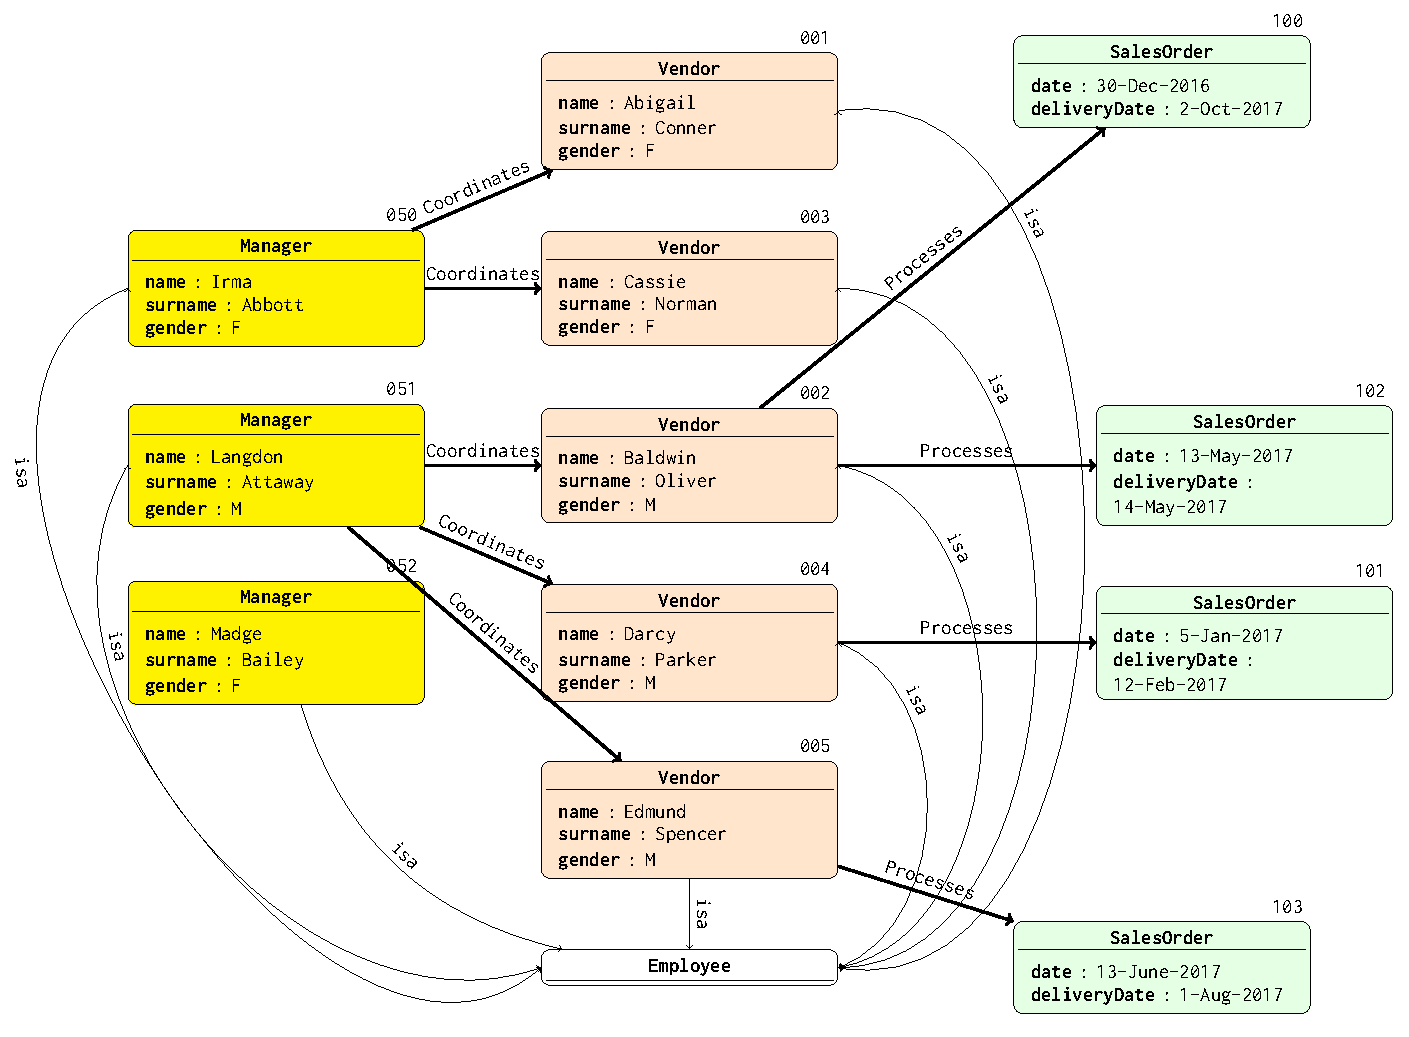
\includegraphics[scale=.6]{fig/02models/06graphWithRDF}
		\subcaption{Representing the generalization within the graph data model through \texttt{isa} edges.}
		\label{fig:graphofISAInstance}
	\end{minipage}
	%\end{adjustbox}
	\caption{Comparing the ability of expressing generalization between the relational model and property graphs. }
	\label{fig:relationalinstance}
\end{figure}

\paragraph*{Generalization and Inheritance}
Another feature of the Entity Relationship model is the ability of expressing generalizations, through which we could state out that an entity could be derived from another one (similarly to subclassing in object oriented programming). Such generalizations\index{is a} are modelled within the ER model through \texttt{ISA}\index{is a} triangular nodes as the one in Figure \vref{fig:erISA}, extending the previous ER diagram in Figure \ref{fig:erschema}. In particular, we want to distinguish two different kind of \texttt{Employee}s, the \texttt{Vendor}s and the \texttt{Manager}s, having different tasks: the \texttt{Manager}s administer the \texttt{Vendor}s, which could process the \texttt{SalesOrder}s. As we could observe from Figure \ref{fig:instanceRemovesIsa}, there could be ER model instantiations in the relational model that remove such explicit information for efficiency reasons, as explained in the following example:

\begin{example}
Instead of using just two distinct relations as in Figure \ref{fig:instanceRemovesIsa}, \texttt{Vendor} and \texttt{Manager}, with the following schemas:
\[Vendor(\underline{\texttt{id}},\texttt{name},\texttt{surname},\texttt{gender},\texttt{manager})\]
\[Manager(\underline{\texttt{id}},\texttt{name},\texttt{surname},\texttt{gender},\texttt{department})\]
we could have used the following schema, preserving the \texttt{isa} generalization:
\[Employee(\underline{\texttt{id}},\texttt{name},\texttt{surname},\texttt{gender})\]
\[Vendor({\texttt{employee\_id}},\texttt{manager})\quad Manager({\texttt{employee\_id}},\texttt{department})\]
This representation comes with the following computational price: if we want to retrieve the personal informations' for each \texttt{Vendor} and \texttt{Manager}, we must always perform join queries while, in the previous cases, we could simply access the \texttt{Vendor} and the \texttt{Manager} tables using the following SQL queries:
\begin{lstlisting}[language=SQL,mathescape=true]
SELECT id, name, surname, gender, manager
FROM Employee, Vendor
WHERE id = employee_id
\end{lstlisting}

\begin{lstlisting}[language=SQL,mathescape=true]
SELECT id, name, surname, gender, department
FROM Employee, Manager
WHERE id = employee_id
\end{lstlisting}

Such SQL queries could be respectively expressed in Relational Algebra as follows:
\[\pi_{\texttt{id},\texttt{name},\texttt{surname},\texttt{gender},\texttt{manager}}(Employee\Join_{\texttt{id}=\texttt{employee\_id}}Vendor)\]
\[\pi_{\texttt{id},\texttt{name},\texttt{surname},\texttt{gender},\texttt{department}}(Employee\Join_{\texttt{id}=\texttt{employee\_id}}Manager)\]

\end{example}

On the other hand, graph databases allow to maintain the \texttt{isa} relation as metadata \cite{Lassila1999} information, because both data and metadata could be expressed within the same graph database instance\footnote{This property will be also later on important for expressing data integration tasks.} \cite{Vasilyeva13}. Figure \ref{fig:graphofISAInstance} shows how to associate metadata (the \texttt{Employee} information with the \texttt{isa} edges) within the original graph data, so that the \texttt{isa} information could be traversed only when required. It is also showed that accessing to such information through graph traversal queries (\textit{path joins}) is more efficient than traversing relations through relational joins. As an example, within a graph database we could retrieve the subgraph containing all the Vendors with their Managers with the following Cypher query:

\begin{lstlisting}[language=Cypher]
MATCH (vendor:Vendor)-[:isa]->(:Employee)<-[:isa]-(boss:Manager)
MATCH path = (vendor:Vendor)-[:hasManager]->(boss:Manager)
RETURN path
\end{lstlisting}

After rewriting the Property Graph model into the RDF graph model as described in \cite{DasSPCB14} (see Section \vref{sec:rdfmodel}), we could express the same query in SPARQL as follows:

\begin{lstlisting}[language=SPARQL,mathescape=true]
PREFIX company: <http://company.com/graphdb#>
CONSTRUCT { 
	?vendorid company:name ?vname;
	          company:surname ?vsurname;
	          company:gender ?vgender;
	          company:hasManager ?managerid.
	?managerid company:name ?mname;
	           company:surname ?msurname;
	           company:gender ?mgender;
	           company:department ?dept.
} WHERE {
    company:Vendor a company:Employee.
    ?vendorid a company:Vendor;
	          company:name ?vname;
	          company:surname ?vsurname;
	          company:gender ?vgender;
	          company:hasManager ?managerid.
    company:Manager a company:Employee.
    ?managerid a company:Manager;
	           company:name ?mname;
	           company:surname ?msurname;
	           company:gender ?mgender;
	           company:department ?dept.
}
\end{lstlisting}

Graph query languages such as Cypher and SPARQL are going to be described in Section \vref{sec:dbqlang}.

\subsection{Representing graphs}
The previous sections showed how relational databases could be completely described by Property Graphs \cite{Neo4jAlg}.  We could formalize the data structure used in Figure \ref{fig:graphofdb1} as follows:

\begin{definition}[Property Graph]\label{def:propg10}
A \textbf{property graph}\index{graph!property graph|textbf} is a tuple $(V,E,L,A,U,\ell,\kappa,\lambda)$, such that $V$ and $E$ are sets of distinct integer identifiers ($V\subseteq \mathbb{N}$, $E\subseteq \mathbb{N}$, $V\cap E=\emptyset$). $L$ is a set of labels, $A$ is a set of attributes and $U$ a set of values.

Concerning the functions, $\ell\colon V\cup E\to \mathcal{P}(L)$ is a function associating to each vertex and edge of the graph a set of labels\footnote{I prefer to associate to each vertex and edge a set of labels instead of one single label in order to be able to express the Neo4J \cite{Neo4jMan,Neo4jAlg} each vertex and edge could have more than one possible label}; $\kappa\colon V\cup E\to A\to U$   is a function associating, for each vertex and edge within the graph and for each attribute within $A$, a value in $U$; last, $\lambda\colon E\to V\times V$ is the function associating to each edge $e\in E$ a pair of vertices $\lambda(e)=(s,t)\in V\times V$, where $s$ is the source vertex and $t$ is the target. 
\end{definition}

Given the data model provided by this definition, we can now istantiate 
the graph illustrated in Figure \ref{fig:graphofdb1} within this very model as showed by the following example:

\begin{example}
Graph in Figure \ref{fig:graphofdb1} is described by the following vertex set:
\[V=\{\texttt{001},\texttt{002},\texttt{003},\texttt{004},\texttt{005},\texttt{100},\texttt{101},\texttt{102},\texttt{103},\texttt{500},\texttt{501},\texttt{502},\texttt{503}\}\]
The label association is defined as follows:
\[\ell(\texttt{001})=\ell(\texttt{002})=\ell(\texttt{003})=\ell(\texttt{004})=\ell(\texttt{005})=\{\texttt{\textbf{Employee}}\}\]
\[\ell(\texttt{100})=\ell(\texttt{101})=\ell(\texttt{102})=\ell(\texttt{103})=\{\texttt{\textbf{SalesOrder}}\}\]
\[\ell(\texttt{500})=\ell(\texttt{501})=\ell(\texttt{502})=\ell(\texttt{503})=\{\texttt{\textbf{Product}}\}\]
Moreover, we could model the edges as follows:
\[E=\{\texttt{800},\texttt{801},\texttt{802},\texttt{803},\texttt{804},\texttt{805},\texttt{806},\texttt{807},\texttt{808}\}\]
Even the edges could show labels as follows:
\[\ell(\texttt{800})=\ell(\texttt{801})=\ell(\texttt{802})=\ell(\texttt{803}=\{\textbf{\texttt{Processes}}\}\]
\[\ell(\texttt{804})=\ell(\texttt{805})=\ell(\texttt{806})=\ell(\texttt{807}=\ell(\texttt{808}=\{\textbf{\texttt{ComposedOf}}\}\]
In this scenario, edges do not have associated attributes or values, and hence could be modelled as relational tuples with $0$ arity. Edges' sources and destinations are modelled through the $\lambda$ function:
\[\lambda(\texttt{800})=(\texttt{002},\texttt{100})\quad \lambda(\texttt{801})=(\texttt{002},\texttt{102})\quad \lambda(\texttt{803})=(\texttt{004},\texttt{101})\quad \lambda(\texttt{804})=(\texttt{005},\texttt{103})\dots\]

In particular, the properties and the values can be associated to both vertices and edges. For example,  \texttt{Employee} \textit{Abigail Conner} is modelled as follows:
\[\kappa(\texttt{001},\texttt{name})=\textit{Abigail}\quad \kappa(\texttt{001},\texttt{surname})=\textit{Conner}\quad \kappa(\texttt{001},\texttt{gender})=\textit{F}\] 
while the association between \textit{Coffee} and the first \texttt{SalesOrder} in chronological order is modelled with the following properties:
\[\kappa(804,\texttt{quantity})=1\]

\end{example}


